\chapter{Introducción y objetivo}
\label{ch:introduccion}

La realidad aumentada es una tecnología que está en pleno auge, no paramos de ver noticias que nos muestran todo lo que esta permite, las diferentes utilizades que tiene y como va a mejorarnos la vida. No obstante esto no era así hace un año, como se puede observar en el grafico del "Hype Cycle" de Gartner sobre tecnologías emergentes en 2017, Figura \ref{figura-gartner}, la realidad aumentada se situaba en el tramo de desilusión, lo que significa que apenas se hablaba de dicha tecnología, y todavía habia mucho trabajo para que saliera adelante.\\

\begin{figure}[h]
  \centering
  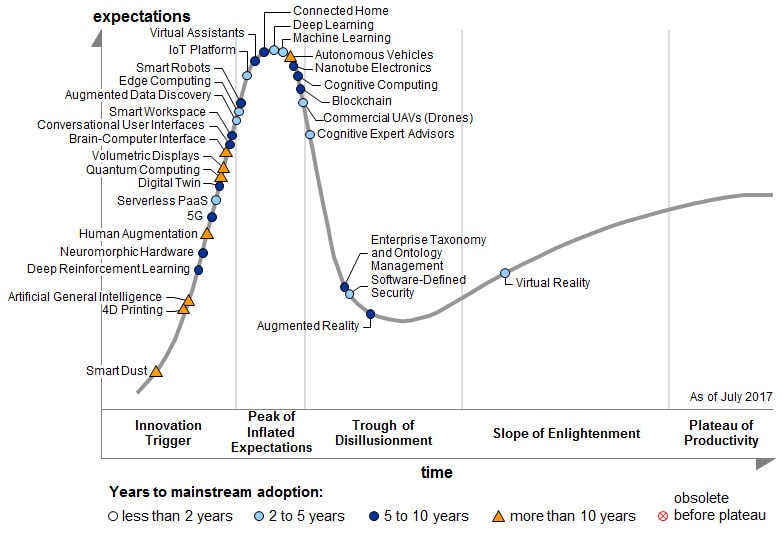
\includegraphics[scale=0.4]{gartner-hype-cycle}
  \caption{Imagen que muestra el "Hype cycle" de Gartner para tecnologías emergentes en 2017.\protect\footnotemark}
  \label{figura-gartner}
\end{figure}

\footnotetext{ \url{https://www.gartner.com/newsroom/id/3784363}, Gartner (July 2017)}

Sin embargo, desde que Apple y Google lanzaran sus respectivas librerías hace apenas un año, la realidad aumentada ha mejorado su situación notablemente, distanciándose de la realidad aumentada vista hasta el momento, estas nuevas librerias permiten, con los componentes de un dispositivo móvil de masas sea posible reconocer y entender el mundo que le rodea, así como su posición en el mundo. Esto supone una diferenciación en las tecnologías hasta entonces presentes, que o bien necesitaban de mucho hardware para ser capaces de conseguir esto, o en dispositivos móviles de masas, tenían capacidades reducidas.\\

Actualmente la realidad aumentada abre un mundo de grandes posibilidades que pueden revolucionar muchos ámbitos, entre ellos el de los juegos. Un videojuego ya no tiene que quedarse dentro de una pantalla o un mundo virtual, ahora puede dar el salto el mundo real, esto aporta un grado de realismo y espectacularidad que puede suponer una reinvención de los juegos como ahora los conocemos.\\

Por otro lado, la mayoría de la población dispone de un dispositivo móvil, como podemos ver en la Figura \ref{figura-ine}, en el año 2017, un 97.4\% de los hogares españoles contaba con al menos un dispositivo móvil \cite{ine}, esto implica que casi la totalidad de los españoles tiene acceso a dispositivos móviles, y por tanto, a las aplicaciones que utilizan realidad aumentada.

\begin{figure}[h]
  \centering
  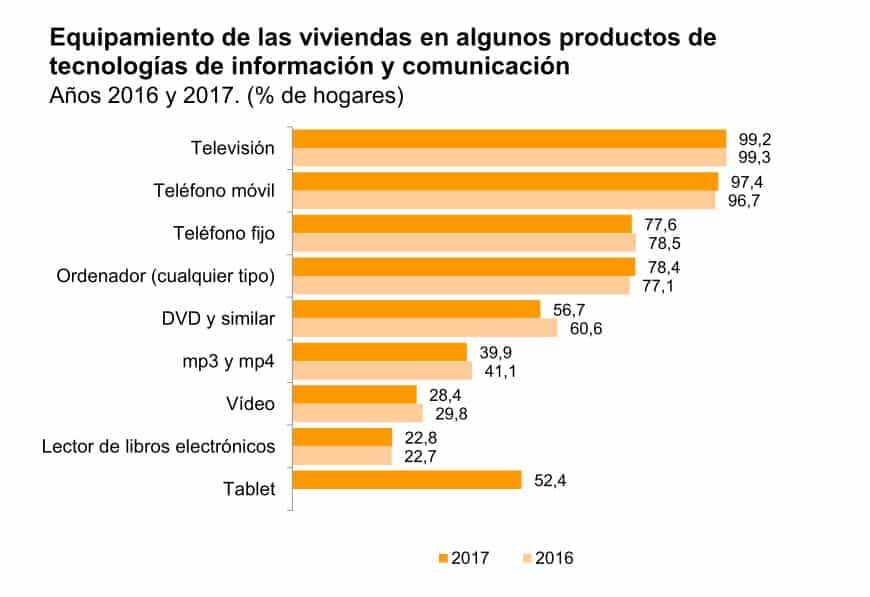
\includegraphics[scale=0.37]{ine2017}
  \caption{Imagen que muestra los porcentajes de hogares que cuentan con cada dispositivo tecnológico.\protect\footnotemark}
  \label{figura-ine}
\end{figure}

\footnotetext{{\em Encuesta sobre Equipamiento y Uso de Tecnologías de la Información y Comunicación en los Hogares.} INE, B. (2017).}

\newpage

\section{Motivación}
Personalmente el estar una gran parte del tiempo de cada dia utilizando mi teléfono móvil y jugando con el me despertó la curiosidad acerca de como se desarrollan los videojuegos, y que es lo que hay detras del producto que al final el usuario descarga de una tienda de aplicaciones.\\

Por otro lado, mi interés por el desarrollo del software me lleva a querer conocer y explorar este mundo, la experiencia de planificar y desarrollar un proyecto software al completo por mi mismo.\\

Las nuevas tecnologías siempre me han llamado la atención y me gusta estar informado sobre ellas, y viendo la revolución de la realidad aumentada me pareció un mundo apasionante por las capacidades ofrece, el poder fusionar el mundo virtual y real, y llevar a cabo aplicaciones y juegos con ella, me pareció algo fascinante y que sin duda me gustaría explorar.\\

La amplia disponibilidad de dispositivos móviles entre la población, y el alto nivel de uso diario que hacen los usuarios de estos, hace del desarrollo para estos dispositivos algo atractivo, ya que es probablemente la mayor plataforma para desarrolladores de software actualmente.\\

Esto en conjunto con el crecimiento de la realidad aumentada, hace que un juego para dispositivos móviles que hace uso de esta tecnología, sea una opción muy interesante para un proyecto, que permite adquirir conocimientos en el desarrollo de videojuegos, en el desarrollo de aplicaciones móviles, y exploarar la realidad aumentada y lo que puede aportar a las aplicaciones de dispositivos móviles actuales.

\section{Estructura del documento}
Este documento se divide en 7 capítulos, a continuación se detalla el contenido de cada uno de los capítulos del documento:
\begin{itemize}
  \item \textbf{Capítulo 1, Introducción y objetivo:} En este capítulo se hace una pequeña introducción al proyecto, explicando la motivación por la que surgió el proyecto, la estructura del documento, y también se exponen los objetivos que han sido establecidos para este proyecto.
  \item \textbf{Capítulo 2, Estado del arte:} En este capítulo se hará una exposición de cual es el estado actual de la realidad aumentada, diferencias con tecnologías similares, que aplicaciones tiene, varios estudios de mercado, etc. En resumen, este punto pone al lector en contexto de la situación actual de la realidad aumentada.
  \item \textbf{Capítulo 3, Análisis inicial del problema:} En este capítulo expondrá la idea inicial del juego, junto con su narrativa.
  \item \textbf{Capítulo 4, Metodologías a usar en el proyecto:} En este capítulo se explica la utilización de metodologías ágiles, del diseño centrado en el usuario y del funcionamiento del desarrollo de videojuegos.
  \item \textbf{Capítulo 5, Plan de entregas:} En este capítulo se detalla el plan de entregas llevado a cabo, y las historias de usuario realizadas para definir los requisitos que tendrá el sistema.
  \item \textbf{Capítulo 6, Desarrollo. Entregas e iteraciones:} En esta capitulo se recogerá el trabajo realizado durante las diferentes iteraciones, así como el resultado de las distintas entregas.
  \item \textbf{Capítulo 7, Conclusiones y Trabajos Futuros:} En este capítulo se expone el resultado del proyecto, las conclusiones obtenidas del desarrollo de éste y los trabajos futuros a realizar en el proyecto.
\end{itemize}

\section{Objetivo}
El objetivo principal de este proyecto es explorar que ventajas puede aportar la realidad aumentada, mas concretamente el SDK ARCore, a los juegos en dispositivos móviles, y mas específicamente a los juegos de mesa en dispositivos móviles. Por tanto, mediante este proyecto se adquirirá experiencia en el desarrollo con tecnologías de realidad aumentada.\\

Una vez mencionado el objetivo principal del proyecto vamos a detallar los objetivos mas específicos:
\begin{itemize}
  \item Investigar una implementación para juegos de mesa virtuales que aporte un enfoque diferente al habitual.
  \item Aprender a planificar y desarrollar proyectos de software utilizando metodologías de desarrollo ágil.
  \item Aprender a desarrollar videojuegos utilizando la herramienta Unity.
  \item Adquirir conocimientos sobre la realidad aumentada y como ésta funciona.
  \item Analizar cuales son los SDK disponibles para desarrollar aplicaciones de realidad aumentada en dispositivos móviles y cuales son las diferencias entre estas.
  \item Aprender a utilizar ARCore para crear experiencias de realidad aumentada.
\end{itemize}
